\documentclass{report}
\usepackage[utf8]{inputenc}
\usepackage{color}
\usepackage{stmaryrd}

\newcommand{\tristan}[1]{\color{red}{TG: #1}\color{black}}
\title{Stream summarization for connected objects}
\author{BO LI }

\usepackage{natbib}
\usepackage{graphicx}
\graphicspath{ {images/} }

\begin{document}

\maketitle

\chapter{Introduction}

\chapter{Related Work}

\section{Introduction}

As we know, we need to process data stream timely due to its volume and velocity. We may lose the opportunity to process them at all, if we did not do it in real time.

https://www.sciencedirect.com/science/article/pii/S1389128610001568

\section{Stream Summarization Problems}

\subsection{Overview of Stream Problems and Algorithms}

The review paper in~\cite{kejariwal2015real} discusses various stream analytic problems and some general techniques for data reduction and synopsis construction. It also gives an overview of streaming platforms developed over the last decade. It identifies 17 classes of streaming algorithms among which sampling, filtering, correlation, etc. 

Most data stream analysis algorithms rely on data reduction and synopsis construction techniques to compute approximate solutions that work with limited storage and time. The paper in~\cite{kejariwal2015real} identifies the following data reduction and synopsis construction techniques: 
\begin{quote}
\begin{itemize}
    \item  \textbf{Sampling} captures the essential characteristics or sub-sample of a data stream.
    \item \textbf{Sliding windows} prevent stale data from influencing analysis and statistics. They also serve as a tool for approximation, given bounded memory~\cite{kejariwal2015real}.
    \item \textbf{Clustering} algorithms separate all points into different groups and make sure that the points in one group as similar as possible, the points in different group as different as possible. For instance, they can be applied to problems such as the k-median problem~\cite{kejariwal2015real}. 
    \item \textbf{Sketches}, introduced by Alon et al~\cite{alon1999space}, summarize data stream using a small amount of memory. The sketch is used to estimate the answer to certain queries (typically, "distance" queries) over a data set~\cite{kejariwal2015real}.
    \item \textbf{Histograms} approximate the distribution of a set of values $v_1, ..., v_n$ by a piecewise constant function $\hat{v}(i),$ so as to minimize the sum of squared error. Equi-width histograms partition the domain into buckets such that the number of $v_i$ values falling into each bucket is uniform across all buckets. End-biased histograms maintain exact counts of items that occur with frequency above a threshold, and approximate the other counts by a uniform distribution~\cite{kejariwal2015real}.
    \item \textbf{Wavelet coefficients} are projections of the given signal (set of data values) onto an orthogonal set of basis vectors. The coefficients have the desirable property that the signal reconstructed from the top few wavelet coefficients best approximates the original signal in terms of the L2 norm~\cite{gilbert2002fast}. The choice of basis vectors determines the type of wavelets.
\end{itemize}
\end{quote}

For each problem in streaming research, there are many algorithms to solve or estimate it. The remainder of this chapter presents certain algorithms used in specific streaming analysis problem.

\subsection{Sampling data}

When the data is huge and we cannot save it into working storage, so we would to sampling data from the whole data stream, then estimating the result base on fraction of the sample and whole data.

But there are some trick in it. for instance, when we would like to query "What fraction of the typical user's queries were repeated over the past month?", the common idea to sampling is extract the for example 1/10 data from the whole stream. but it's not correct for this situation~\cite{leskovec2014mining}.

If there is a repeat data in the data stream, and we extract the sample with the method mention above, then the probability of repeat for this data in sample is 1/10 * 1/10 (first time appear is 1/10, the second appear also need 1/10). so the result of above way is wrong.

Another idea is to select 1/10 users from whole data (the problem is user query on the website), and make 10 buckets, using hash function(result 0-9) if the h(user) = 0 then save the data which sent by this user. Note that we don't need to save user identifiers as they will be hashed consistently to the same bucket.

After that we create a hash function that hash the key into [0, B-1 ] 
and make a parameter t as threshold which initial is B-1, and if the data we saved is bigger than space, we reduce t into t-1(or smaller) and  delete the date whose hash(key) bigger than t-1.
\cite{leskovec2014mining}

In practice, sampling can help to save energy on connected objects. For instance, when we would to do some query on stream, we can estimate the result after sampling from whole stream. We need less communication with objects, because we only need just a part of whole stream to estimate result.  

\subsection{Filtering Stream}

In this situation, we are interested only in particular elements in the stream. For instance, we have a list of email addresses we would like to receive from, but there are 80\% spam, so we need to filter the data to transmit only the non-spam addresses. 

For instance, in a connected Object, it has sensor produce longitude and latitude and others value like temperature, the pace of speed ..., but in some case we only receive data from specific longitude and latitude, so we need to filter the data stream to transmit just what we would like.

The idea is to hash each email address in the list, and put them into a bit array. When we get the result of hash function we change the bit into 1 in bit array for corresponding location, after hashing we get the bit array. When a new email comes, we hash the email address and check if the bit is 1 in that corresponding location. If it's than can access, otherwise it's filtered.

\subsubsection{Bloom filter}

The Bloom filter consists of:\cite{leskovec2014mining}
\begin{enumerate}
    \item An array of n bits, initially all 0’s.
    \item A collection of hash functions $h_1, h_2, ... , h_k$. Each hash function maps "key" values to n buckets, corresponding to the n bits of the bit-array.
    \item A set S of m key values.
\end{enumerate}

For each key in set S hash them into bit array, then if a new data coming in we can know that if it has presented or not. If the result of hashing new coming data is 1 in bit array, it means this element has presented before, Otherwise, we make the corresponding bit in array to 1.

So we can say that hashing a key into a given bit, the probability is 1/x, the probability do not hit the given bit is 1-1/x = (x-1)/x.
if all key in set S do not hit the given, the probability is $(\frac{x-1}{x})^y$, change it into $(1-\frac{1}{x})^{x(\frac{y}{x})}$, it's approximation 1/e.
So a given bit is not hit, the probability is $e^{-\frac{y}{x}}$, and when we use many hash function to hash the key in set S, it's $e^{-k\frac{y}{x}}$.

After that we get the big array, and when a data come, we hash it using k hash functions and check if all result of the functions is corresponding 1.

If there is a 0 result, the data will be filtered. the probability of a spam data will pass our filtering(all functions return 1) is $(1-e^{-k\frac{y}{x}})^k$\cite{leskovec2014mining}

\subsection{Estimating Cardinality / distinct elements in stream }

Actually, this problem is same with $F_0$ in frequency moments. For this part, there are many method to compute or estimate Cardinality.

\subsubsection{ Traditional method }
In order to counting distinct elements in stream, the traditional point is to store the elements in a set, and when a element coming, check whether this elements has presented already, if not add it into the set.
One of the traditional method to store this elements is using B-Tree, because of its good efficient on search and insert.But using B-Tree structure need more space to save and worse efficient on merging when the datasets is large.

Another traditional method is using bitmap, this method hash every element into a bit array by hash function. If bit is 1, then the element is already presented, otherwise change the bit from 0 to 1. Bitmap is good at merging(just using OR operation), and only need N bit for element x $\in \{1...n\}$, but if the N is large or undefined bitmap is not good choice.

\subsubsection{Linear Counting}
The Linear Counting is supposed in \citep{whang1990linear}, using $O(N_{max})$.
Assuming there is a hash function which can hash elements into m result, if the result bit is 0, then change it to 1. After hashing assume that already rest u bit are 0, then $\hat{n} = -mlog\frac{u}{m}$.

\textbf{Proof:} We define that the result from hash function is independent uniform distribution, so the event $A_j$ the jth bit is 0 after passing n element is $P(A_j) = (1-\frac{1}{m})^n$. Because each bit is independent, so the expectation of u is $E(u) = \sum_{j=1}^{m} P(A_j) = m(1-\frac{1}{m})^n = m((1+\frac{1}{-m})^{-m})^{-\frac{n}{m}}$. $E(u) = me^{-\frac{n}{m}} $. So we final get $n = -m\log{\frac{E(u)}{m}}$

\subsubsection{ Flajolet Martin Algorithm}

Flajolet and Martin~\cite{flajolet1985probabilistic} support an algorithm which using $O(\log n)$ space to estimate Cardinality. 

The main idea of Flajolet-Martin Algorithm is estimating the number of distinct elements by hashing the elements of the data stream into a long enough bit-string. From the hashing function, the more different elements we see in the stream, the more hash values we have in the bit-string, so we will see some "unusual" values, whose ends in many 0's. So we define the R = the maximum number of the 0 in all value's end. We can estimate the number of distinct elements in stream is $2^R$.~\cite{flajolet1985probabilistic}


\subsubsection{LogLog Counting }
This method was presented in \citep{durand2003loglog} which using less space complexity $O(\log\log{N_{max}})$.
Same as LC, LLC need a hash function to hash every element, and the result of hash function are independent uniform distribution and the length of result is constant.
Assuming the length of result of hash function is L, then we need a bit array which has L bit. As assuming above each bit is independent, after hashing a element A, we get a bit array with L length. Defined $\rho(A)$ is the position that the first 1 presents. We can estimate that $\hat{n} = 2^{\rho_{max}}$.

\textbf{Proof:} Because every bit in bit array is independent, so after hashing n element, the probability of not result X bigger than $K = \rho_{max}$ is $P_n(X\leq k) = (1-\frac{1}{2^k})^n$, and the probability that at least one result X bigger than or equal $K = \rho_{max}$ is  $P_n(X\geq k) = 1-(1-\frac{1}{2^{k-1}})^n$.

From above we can learn that when $n \ll 2^k, P_n(X\geq k) \approx 0$. Opposite, if $n \gg 2^k, P_n(X\leq k) \approx 0$, So $2^{\rho_{max}}$ can be a estimation for Cardinality Counting.


\subsection{Frequency moments}

The problem, called computing “moments,” involves the distribution of frequencies of different elements in the stream. So from moments we can learn some characteristic by computing moments, $F_0$ is the number of distinct elements in data, $F_1$ is the number of elements in the data, $F_2$ presents the surprise index of data stream, In general, $F_k$ represents the degree of skew in the data.


Generally, $k_{th}$Frequency moments of a set of frequencies \textbf{a} is defined as $F_k(a) = \sum_{i=1}^n a_i^k $.

In data stream we can define it as follow: 

Let A = $(a_1,a_2,...,a_m)$ be a sequence of elements, and the $a_i$ is a numbers of N = {1,2...,n}. Let $m_i = |{j:a_j = i}|$, the frequency moments k$\geq$0, $F_k = \sum_{i=1}^{n}  m_i^k$.
 
 
Define that the sequence have m data and $a_m$ = {1...n}, the relative error is $\lambda$ and the error-probability is $\epsilon$


\subsubsection{ Estimating $F_k$}
Base on they mentioned, consider the members of N as elements of the finite field $F = GF(2^d)$ (what's GF())
for every $c > 2$ the ratio between the estimation Y and $F_0$ is not between $\frac{1}{c}$ and c, is smaller than $\frac{2}{c}$.


For estimate $F_k$ we define $s_1 = \frac{8kn^{1-\frac{1}{k}}}{\lambda^2}$, $s_2 = 2log(\frac{1}{\epsilon})$
the algorithm computes $s_2$ random variables $Y_1,...Y_{s_2}$ and output their median Y. For each $Y_i$ is the average of $s_1$ random variables $X_{ij} : 1\leq j \leq s_1$ (which means $m(r^k-(r-1)^k)$). So for each $Y_i$ we need $s_1$ X, we total need $s_2$ Y, so we need $s_1 \times s_2 (\log n + \log m)$ (save the value and count). And they make sure $prob[|Y_i - F_k > \lambda F_k|] \leq \epsilon$.

\subsubsection{$F_0$ / Distinct elements counting}

For $F_0$(count distinct element) please see the chapter "Estimating Cardinality".

\subsubsection{ AMS algoritm for $F_2$ / surprise index}


 In~\cite{alon1999space} the main idea is how to estimate the frequency moments in data stream and consider the space complexity.

For estimating F2(surprise index) the method is almost same as how to estimate $F_k$ which before mentioned but the space complexity is $O(\sqrt{n}(\log n + \log m))$.

Note: what's four-wise independent, what's $GF()$.


\subsection{Cardinality estimation over Sliding window}
There are already several method to estimate cardinality of a data stream, for instance, Flajolet Martin algorithm, AMS algorithm, Liner count algorithm etc. But in practical, we only would like to concentrate on the stream data during a certain period, so the model called sliding window has been used. The stale data should be evicted from storage in this model. So, how to do cardinality estimation over sliding window is also a challenge. The main difficult points are which structure should be used to record the data and the times it emerges, and how to update aging level of data and evict it from our sliding window. Several method has been proposed over the past decade, we will introduce them in next section.

\subsubsection{Sliding HyperLogLog algorithm}

This algorithm has been proposed by Chabchoub et al.~\cite{chabchoub2010sliding}. It extends the HyperLogLog~\cite{flajolet2007hyperloglog} algorithm over sliding window. 
\subsubsection{Introduct hyperLogLog}
HyperLogLog is a improved version from LogLog count algorithm ~\cite{durand2003loglog} which estimates cardinality by hashing each stream data into a bit array and record the position of first 1's bit in bit array, then estimating the cardinality using formula $\hat{n} = 2^{\rho_{max}}$ where $\rho_{max}$ 
where $\rho_{max}$ is the max first 1's position number among all bit array ~\cite{durand2003loglog}. In order improve accuracy, LogLog separates data into m buckets where $m = 2^b$ and using the first b bit of bit array to determine which bucket the data belong to. Then replace the $\rho_{max}$ in formula with the geometric mean among biggest first 1's positions in each bucket. But geometric mean is very sensitive on discrete value, and the bucket may be empty if the number stream data is not quite a lot. The accuracy of LogLog count method would not be ideal if the size of datasize is not so much~\cite{durand2003loglog}. HyperLogLog solves this problem by using harmonic mean in stead of 
geometric mean, So the algorithm of HyperLogLog as follow:

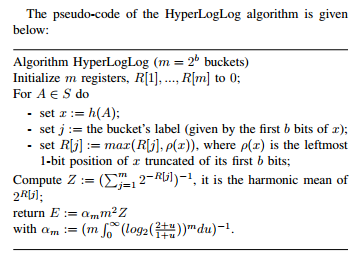
\includegraphics{HyperLogLog.png}

\subsubsection{Sliding HyperLogLog}
In sliding HyperLogLog algorithm, for each data we represent it by pair $<t_i, R_i>$~\cite{chabchoub2010sliding} where $t_i$ is the arrival time stamp of data, $R_i$ is the position of the first 1's bit. In order to get biggest $R_i$ in each bucket, this pair need to be store in buckets~\cite{chabchoub2010sliding}. Once a new data $<t_k, R_k>$ coming, at first deleting old data where $t_i < t_k - W$ where W is the window size, and delete all data where $R_i \leq R_k$, finally add this new data into bucket~\cite{chabchoub2010sliding}. In this algorithm authors using time stamp to manage stream data in slidling window, and using simple pair structure to represent data in order to save memory space. 

\subsubsection{Counter Vector Sketch (CVS)}
In the paper ~\cite{shan2016cvs}, Shan et al. described a Sketch based on bitmap sketch also called Liner count~\cite{shan2016cvs} algorithm for estimating cardinality over sliding window. Information about Liner Count algorithm is in section 2.2.4 . As discussed in the paper, CVS is consisted of a a vector of counters V[1]...V[m],each V[i] called entry and each counter of entry in the range from 0 to a certain value C. After hashing data into a entry of vector, the counter would be set as C, and if there is no more data hashed into this entry, the counter should be decreased to be 0~\cite{shan2016cvs}. Once a counter become 0, then the information in that entry will be evicted from memory.
In paper, the certain $C = W*\frac{k}{m}$. Assuming that the size of window is W, size of vector of CVS is m, if k entries would be hit uniformly and independently in unit time, the probability of V[i] be hit in time i is $\frac{k}{m}$. Supposing an entry is hit $K_w$ times in W unit times, then $Mean(k_w) = \sum_{i}^{W}E(entry be hit) = \sum_{i}^{W}(\frac{k}{m}) = \frac{W*k}{m}$~\cite{shan2016cvs}. It means each counter is reduced by $\frac{W*k}{m}$ during W unit times on average. So the maximum value of the counter C is $\frac{W*k}{m}$.According this theorem, CVS will random select k entries, and if the counter of entry is greater than 0, it would be decreased by 1. CVS estimates cardinality according the number of 0 in vector which same as Liner count algorithm, but it using a counter to reflect the aging level of data. According to the experiment result in the paper ~\cite{shan2016cvs}, CVS sketch achieves high accuracy and also works more efficient than index sketch and Time Stamp Vector sketch.

\subsubsection{LRU-LC}
Another algorithm for estimating cardinality over sliding window, which based on Liner Count algorithm, is LRU-LC ~\cite{shan2016lru} proposed by Shan et al. LRU-LC uses Vector of LRU entries in stead of bit array. All entries constitute a LRU queue which is sorted in time order. Each coming data would be hashing into a LRU entry and also mark a element $\bigtriangleup t$ means the different between time stamp of new data and last data~\cite{shan2016lru}. Follow graph illustrates it clearly.

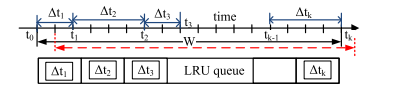
\includegraphics{LRU-LC-dif-time.png}

Using this design, the aging degree of LRU entry could be calculated easily by $D_{aging}[i] = W-\sum_{j=i}^{k}\bigtriangleup t_j$ ~\cite{shan2016lru}. If a hashed LRU entry is inactive -- never be hit by hash function-- then making it active and adding it into tail of LRU queue, because of the time stamp of the newest data is biggest. If hashed LRU entry is already in LRU queue, $LRU.old\bigtriangleup t += \bigtriangleup t$. The LRU entry would be removed from sliding window, once its aging degree equals 0~\cite{shan2016lru}. The pseudocode of LRU-LC algorithm as follow:

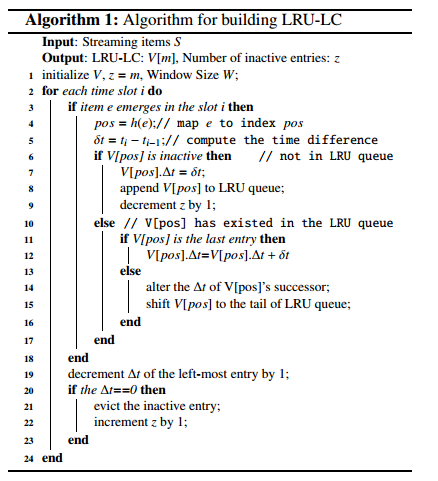
\includegraphics{LRU-LC-ALgorithm.png}

LRU-LC update data's aging degree using different coming time method($\bigtriangleup t$), rather than random select entries to update aging degree in CVS algorithm.



\subsection{Data Stream Clustering}
\subsubsection{CluStream Framework}

In the paper~\cite{aggarwal2003framework} authors discussed a framework using for clustering evolving data streams.
It is called CluStream. This framework have two components, the Online micro-clustering component is used for storage of summary statistic in data steams, these information are computed based on micro-clusters which use \textbf{cluster feature vector}~\cite{zhang1996birch} to cluster data streams.
In online component, Pyramidal pattern is be used to store micro-clusters as snapshots in order to acquire summary statistics over different time horizons. The offline component is designed for analyst, which can present quick understanding of the clusters of data streams with the statistic information from online component and specific input for example what time horizon is using for clustering, how many clusters should data stream be clustering. In the offline macro-clustering component, we can use its \textbf{subtractive} property of the micro-clustering to generate higher level clusters over different time horizons. For instance, the current clock time is $t_c$ and the user wishes to find clusters on a time horizon of length h, then we can find the snapshot in $t_c$ and $(t_c - h)$ then we can get the clusters with time horizon of length h. It is not possible to save snapshots for every moment, so this framework using pyramidal time frame to storage snapshots with different orders. The order of a class of snapshots means that the level of granularity in real time.


\subsection{Data Stream Classification}

\subsubsection{Hoeffding trees and Very Fast Decision System}

Classic Decision Tree is a basic method of data mining, it has been widely used in supervised classification. Because of increasing size, the Classic decision tree will be created with many levels, and may fail if the volume of data is infinite. In the learning process the data may can only read once, so quick response is needed. As we known that Information Gain and Gini index are using to decide which attribute is the best one to split, so we split the training data on this attribute. The Hoeffding tree~\cite{domingos2000mining} designed by Pedro and Geoff, using only a small subset of whole training data to decide the best attribution to split training data. Hoeffding tree use Hoeffding bound to calculate the how many data is needed for determine the best attribute. The pseudo-code of Hoeffding Tree is In "Table 1".

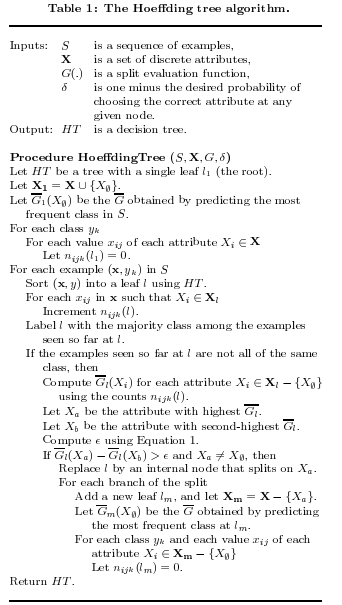
\includegraphics{HoeffdingTree.png}

VFDT System us a decision tree learning system based on Hoeffding tree. It is able to compute attribute evaluation measure with either information gain or Gini index. 

VFDT using constant time and memory space to process each example data, and it uses Hoeffding bounds to make sure that the result using subset training data is close the result with whole training data. From the expirment of Pedro and Geoff~\cite{domingos2000mining}, VFDT is using to mining the stream of Web page requests, and finally VFDT system works better than C4.5 decision tree.
Because of many case of evolution of stream data over time, a method called CVFDT~\cite{jin2003efficient}, which using sliding windows over the VFDT, is presented. It makes sure the data in sliding windows are latest and updated classifier when the newest data coming in.


\subsection{ Counting 1's in a Window}
In this situation, suppose we have a window of length N on a binary stream. We would like to find out "how many 1's are there in the last k bit" in any time.(k $\leq$ N).

For this query problem, if we want to compute the result exactly, we need to know the all data in N bits.

\subsubsection{Datar-Gionis-Indyk-Motwani ALgorithm / Estimating}
We can estimate the result using DGIM algorithm. This version of the algorithm uses $O(\log^2{N})$bits to store the Window of N bits, and we can estimate the result in the window with an error of no more than $50\%$.
For each data from stream, it has timestamp for itself, we represent timestamps modulo N, so we can store each data using $\log{2}{N}$ bits. Then we divide the window into buckets, consisting of: (1) the timestamp of right end data. (2) The number of 1's in the bucket. This number must be a power of 2, for the number of 1's = $2^j$, we can only store the j using $O(\log\log{2}{N})$.($2^j\leq N , j< \log N$, using binary bit to store j).

Because the number of buckets is $O(\log{2}{N})$(all bit is 1), so the total space required for all the buckets representing a window of size N is $O(\log^2{N})$.

\section{Data Mining in Sensor data}
\subsection{Events and Event Processing}

\todo{Introduce this section by summarizing the difference between events and stream processing. Give an example.}
\todo{https://softwareengineeringdaily.com/2016/02/04/stream-processing-vs-complex-event-processing/}

We can categorize events as atomic events and composite events. Atomic~\cite{chakravarthy1994composite} events be also known as primitive events which is the smallest event in a system, only occur at specific time point or even not occur. Composite events known as complex events is comprised of atomic events and other composite events.The atomic event only occur at a point of time, but the composite event can last for a long time, for instance interval event~\cite{chakravarthy1994snoop}.In any event, there are many attribute, they may be certain or uncertain. It is called uncertain event if an event has one or more uncertain attributes, otherwise it is certain event. There is a special case, an event is called non-spontaneous event~\cite{garofalakis2006probabilistic} because it cannot detect occurrence by itself only when it is queried or expired. Such non-spontaneous events~\cite{wang2006bridging}, for instance negated events, can be produce by RFID application and sensor application. Each event contains its properties for instance time, location, identification and others information of event~\cite{aggarwal2013managing}. These properties is named event context, which is important for event processing and can process events more efficient.


In generally, we cannot know or predict exactly an event will happen or not~\cite{chandy2009event}. So the purpose of event processing is to make sure that detecting those event in real-time method or in quasi-real-time manner~\cite{aggarwal2013managing}. The event processing process collect the meaningful or valuable data by processing event then perform operations.Thus, event processing applications need lots of functional capabilities like data filtering, pattern detection etc. and non-functional capabilities like performance, response time etc~\cite{aggarwal2013managing}.

It's hard to say what's different between stream processing (SP)~\cite{barga2006consistent} and event processing(EP), because they all can handle the query over the sequence of events. In practical, SP is mainly used to manage on massive data with fewer query action. Oppositely, EP aim to manage the sharing between queries and patterns, and generate corresponding response~\cite{chandy201110201}. 

The Complex event processing (CEP)~\cite{demers2007cayuga} could help us, if the event is too complex. It is used to detect events with specific significant patterns, for instance exceptions, threats, and then generate response in timely fashion~\cite{aggarwal2013managing}.

\subsection{Mining Sensor Data Streams}

There are several problem when Mining Sensor streams

\begin{itemize}
    \item One pass algorithms are needed, because data set is too large to be stored and multiple accessed.
    \item Evolution of the data should be considered when design algorithms, because data may evolve over time.
    \item reduction of uncertainty is important in mining process, since data from sensor maybe uncertain and error~\cite{aggarwal2013managing}.
\end{itemize}

Data from Sensor often produce error in data collection and transmission~\cite{aggarwal2013managing}. A general method could use to solve this problem, called \textbf{model driven data acquisition}~\cite{deshpande2004model}, which could model the uncertain data during receive process.

If the data set is large, several method could be used.
\begin{enumerate}
    \item Decreasing the sampling rate in data collection and transmission~\cite{aggarwal2013managing}. Using this method, we decrease the size of the sub-set of data from sampling, but do sampling frequently to ensure accuracy.
    \item Discarding some parts of the data. For instance, load shedding\cite{aggarwal2013managing}, selecting data points from the streams and dropping unprocessed data in order to reduce the stress of processing. We cannot control the incoming rate of data steams, but we need to be able to adjust the processing rates.
    \item Selecting data from particular sensor in a particular time. It is also used to reduce the power consumption in data collection and transmission. For data selection, we can using filtering technique, to filter the data which we not prefer.
\end{enumerate}

\subsection{Power Reduction in data Collection}

The technique \textbf{sensor selection}~\cite{aggarwal2013managing} is using to reduce the amount of collected data. For instance, there are two sensor is close in physical location, So we can collect the data from only one sensor and predict the data which produce in anther sensor rather than collecting data in both~\cite{aggarwal2013managing}. In our work, we will explore stream summarization instead of sensor selection.

\subsection{Power Reduction in data transmission}

There is a method called In-Network~\cite{aggarwal2013managing} processing which can help to decrease the cost in data transmission. In generally, the raw data generated by sensor will send to
a Central server for processing. Because of the huge amount of data, the transmission will takes lots of energy. In-Network processing technique allocate certain nodes in the network as \textbf{aggregators} which aggregated information from sensors in certain area, and then send these processed data rather than a mass of raw data to central server. In our situation, this In-Network method is not fit, because of all sensor integrate in a board. WHat we need to concern is Power reduction in data transmission between devices via BLE.



\section{Stream mining for connected objects (IoT)}

\subsection{Data mining for the internet of things}

For mining data on IoT, many works have been studied. Gector Gonzalez et al.~\cite{gonzalez2006warehousing} designed a model called RF-Cuboids, which is used to mine RFID stream data \todo{be more specific}. Xiaolei Li et al.~\cite{li2007roam} proposed ROAM, a framework used for  detecting exception in moving object. For sensor data, Rarisa Rashidi et al.~\cite{rashidi2010adaptive} suggested a mining framework base on pattern mining method to mining sensor data~\cite{bin2010research}. Besides these regular method for data mining in IoT, four different data mining model have been proposed in paper~\cite{bin2010research}.
\begin{itemize}
    \item Multi-layer model has four laters\cite{bin2010research}: 
    \begin{enumerate}
        \item Data collection layer which is responsible to collect various data from devices such as GPS data, sensor data, RFID data etc. 
        
        \item Data management layer is used to save and mange collected data.
        \item Event processing layer is incharge for analyze the events in IoT, such as doing some query on data.
        \item Data mining service layer using data minging algorithm ,such classification and clustering, to mining collected data in order to get result which will be using as service in application.
    \end{enumerate}
    This model like regular data mining process, which include data collecting, data pre-processing, and data mining.
    
    \item Distributed model can resolve several issue on data mining in IoT such distributed storage and energy cost in data transmission.
    \begin{enumerate}
        \item Mass data is stored in different place because many devices are configured on different position. So it's easier to mining these data using distributed model.
        \item Requirement of performance is high for centralized devices, if all data need to be processed on center timely. Using distributed model can help reducing press of centralized devices.
        \item Mass energy cost in data transmission if it is needed to send all data to central node.
        \item Data security, data privacy could be guaranteed by using distributed model~\cite{bin2010research}.
    \end{enumerate}
    In this model, sub-node summarize the raw data which is sent from devices, such as filtering, sampling etc. And save the processed data in local storage as local model. These local model will be send to central node, and aggregated as global model~\cite{bin2010research}.
    
    \item Grid based model is using grid resource to do data mining. The main idea of this model is that consider all object in IoT as sources for grid computing~\cite{bin2010research}. According DataMiningGrid~\cite{stankovski2008digging} which from Stankovski V. et al., this model has been proposed, And it can provide many types of hardware and software.
    
    \item Model from multi-technology integration perspective~\cite{bin2010research}, combine several technology to mining data. It using IPV6 and ubiquitous ways to ensure access different internet, such RFID, sensor network, telecommunication nework etc. Trusted control plane~\cite{bin2010research} is used to ensure the correctness and reliability of data transmission.
    
\end{itemize}
\subsection{Power reduction techniques in IoT}

Improve communication protocols: 
http://ieeexplore.ieee.org/abstract/document/926982/
--http://www.mdpi.com/1424-8220/12/9/11734/html
\subsubsection{Overview of BLE(Bluetooth Low Energy) Technology}
In our project, the stream data need to be sent be BLE(Bluetooth Low Energy) which is a emerging wireless technology to using in a short-range communication between devices\textcolor{red}{[1]}. It makes less energy cost than traditional Bluetooth, that's why it's called BLE. This section give a overview of BLE, including BLE protocol stack, and main function in each layer.

There are 2 parts to compose BLE protocol stack:
\begin{enumerate}
    \item \textbf{The Controller} is usually applied on small SOC(System-on-Chip) which include Physical and Link Layer\textcolor{red}{sensor}
    
    \item \textbf{The Host} runs on application processor\textcolor{red}{sensor}, and lots of functionality are used on upper layer which is included in the Host.
\end{enumerate}
The picture blow show BLE protocol stack clearly:

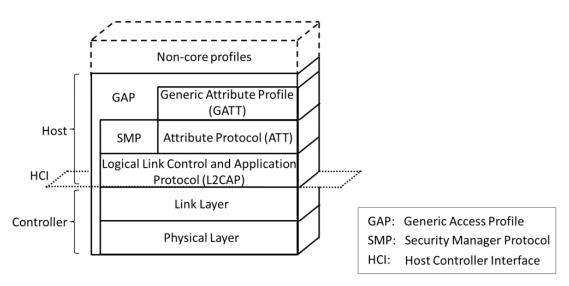
\includegraphics{BLEstack.jpg}

It's worth noting that BLE and traditional Bluetooth are currently incompatible, so If a device contains only one of them, this device cannot be communicated with another one. We call a device \textbf{dual-mode device} if a device supports both of them\textcolor{red}{sensor}. The detail in each layer show blow.

\begin{enumerate}
    \item Physical Layer
        In Physical Layer the data rata is defined as 1 Mbps, BLE defines two type of BLE RF(Radio Frequency) channels: 
        \begin{itemize}
            \item Advertising channel is used for discovering devices, establishing connection and broadcasting data. 
            \item Data channel is used for build bidirectional connection between devices.
        \end{itemize}
        All channels in physical layer use Gaussian Frequency Shift Keying(GFSK) modulation which modulation index is between a range of 0.45 and 0.55. This modulation could reduce power consumption.
        
        In bidirectional communication, devices have to connect to each other. The procedure of connection establishment is like master/slave model, which the slave device(advertiser) announces it is a device by using advertising channel and the master device(initiator) need to listen for advertisements. The master device will transmit a Connection Request Message to slave device, as soon as receiving the advertising packets from slave device, and then the connection is established if master get a good result from slave. 
        
    \item Link Layer
        In Link layer the role of devices are defined for creating connection: master or slave. A slave device can only connect with exact one master device but a master could have many slave.
        Once the connection is created, all packets are transmitting by physical channel with same channel frequency. Connection events are non-overlapping time units of physical channel. The connection events starts with data transmission from master, and the slave must send response packet to master but it's not necessary for master to response slave's packets.
\end{enumerate}    
    In order to save energy, slave will entry sleep mode when there is not packet for it, and wake up periodically to wait for packet.
    




Turn off sensors (sensor selection). Our approach is a compromise between sensor selection and full data transmission.

\subsection{Hardware architectures}

Optimized for object detection: http://ieeexplore.ieee.org/stamp/stamp.jsp?tp=&arnumber=6697982
Look at references inside. 

Instead, we aim at developing general-purpose techniques to save energy during data collection. These techniques should be applicable to any hardware architecture. 

\section{Data Compression in Sensor Network}
In our project, we aim to find  strategies to decrease the number of transmission data  so that reducing the energy consumption in sensor nodes or other IoT devices. So, how to do data compression is also in our research.
There are lots of traditional compression algorithm, for instantce gzip, bzip2 and Lempel-Ziv etc. But most of them are only concentrated on reduction of memory space rather than energy.  Cause running algorithm in microprocessor of devices also need energy, If the complexity of algorithm is high, then more energy might cost than energy saved in transmitting less data~\cite{barr2006energy}. In paper ~\cite{srisooksai2012practical}, authors pointed out that sensor node is composed by sensing unit which is used to obtain events or relevant data, processing unit which contain memory space to process data obtained and communication unit which  is charge of exchanging data among devices. Since, communication unit is main factor of spending energy in sensor nodes work~\cite{barr2006energy}, in-network processing has been introduced which reducing the amount of transmission data by specific aggregation techniques or data compression algorithm in order to reduce radio communication, thus saving energy~\cite{srisooksai2012practical}. 
\begin{itemize}
    \item \textbf{Aggregation techniques} which usually used in dense sensor network need routing algorithms. It only provides coarse statistic, so this technique might lose much of structure in the data~\cite{srisooksai2012practical}.
    \item \textbf{Data compression schemes},some of them were extension of aggregation techniques, rest of them which generally used in sparse topology sensor networks are operated in each local node independently~\cite{srisooksai2012practical}.
\end{itemize}

In paper~\cite{srisooksai2012practical}, Srisooksai et al. classified data compression algorithm in two categories
\begin{itemize}
    \item \textbf{local data compression approach} compress data locally on each sensor node.
    \item \textbf{distributed data compression approach}usually applied in dense sensor networks.
\end{itemize}
\subsection{Local data compression}
local data compression has been classified into two main techniques in~\cite{srisooksai2012practical}: lossless compression algorithm, which do not lose information during compression and depression process and lossy compression algorithm, which may lose some information.
In lossless compression algorithm, there are two type of algorithm: one is based on dictionary approach, another one is based on predictive coding approaches~\cite{srisooksai2012practical}.
\subsubsubsection{Dictionary based lossless compression algorithm}
\subsubsubsection{A simple lossless entropy compression (LEC) scheme}
LEC algorithm is first proposed in ~\cite{marcelloni2008simple} which is a approximated version of exponential-Golomb code~\cite{teuhola1978compression}. In paper~\cite{marcelloni2008simple}, authors measured temperature and humidity by sensors and compressed data by using LEC. It uses very small dictionary whose size is determined by the number of the bits after ADC converter~\cite{marcelloni2008simple}. For instance, in a sensor node, a measure $m_i$ is gained and converted into numeral value $r_i$ represented on R bit by ADC. At each new data point $r_i$, LEC compute the difference of adjacent points $d_i$ = $r_i$ - $r_{i-1}$, in order to compute $d_0$, the $r_-1$ equals the central value among $2^R$. The difference $d_i$ Encoded by entroy encoder, and represented as a bit sequence in 2 parts $s_i | a_i$ , where $s_i$ is the number of the bits needed to represent the difference $d_i$, and $a_i$ represent $d_i$ based on special rule.In the paper~\cite{marcelloni2008simple}, the authors generated the $s_i$ by Huffman coding. Let's say the $n_i$ is the Decimal expression of $s_i$, then  
$n_i = \lceil\log_2(\abs{d_i})\rceil$~\cite{marcelloni2008simple}
and $n_i \leq R$. Then $s_i$ could be generated by searching Huffman code with $n_i$. Table 1 is used in paper~\cite{marcelloni2008simple}. From the table, it support R+1 symbol($s_i$) and each symbol $s_i$ contains $2^{n_i}$ numeral value. 


%At first, for any measure mi is transformed by analog-to-digital converter into a binary representation ri on R bits~\cite{marcelloni2008simple}. The value differences $d_i = r_i - r_{i-1}$. assuming $r_{-1}$ equal control value among possible value in order to compute $d_0$.  Then Representing each $d_i$ with $s_i|a_i$, $s_i$ is computed according to $n_i$ where $n_i = \lceil\log_2(\abs{d_i})\rceil$ which is not bigger than R,$s_i$ is a variable-length binary string generated from $n_i$ by using Huffman code. For $a_i$ part in $s_i|a_i$, when $d_i>0$, $a_i$ is  $n_i$ low-order bits of two’s complement of $d_i$. $d_i<0$ , $a_i$ is $n_i$ low-order bits of the two’s complement of $(d_i - 1)$. When $d_i =0$, $s_i$ is 00 and $a_i$ is not presented.~\cite{marcelloni2008simple}

In order to operating this algorithm, it’s necessary to save the table in to memory. when a new data $r_i$ come, we need to compute the $d_i$ at first, and then represent the $d_i$ to $s_i|a_i$ with searching table.


%Due to limited resourses in IoT devices, the power saving is need to extend the work life of devices. LEC is a lossless comprssion method, In the paper~cite{marcelloni2008simple}, the authors generated the $s_$ by Huffman coding. Let's say the$n_i$ is the Decimal expression of $s_i$, then $n_i$ = \lceil \log_2^(\mid d_i \mid) \rceil$


\chapter{Our work}
We are working on doing summarization of data stream of sensors which integrate in Neblina Model V2(a standalone 3D orientation tracking module). It uses BLE or COM port to connect other devices.

\section{The Neblina}

Sensors, RAM, sampling frequency, network characteristics.

How much power is required to transmit 10B? 

\section{A basic stream mining technique to save energy}

\subsection{Method}
For data set, we get Quaternion data stream from Neblina, in order to find the relation between window size and threshold, we only rotated Neblina in 2D plane to make sure the data around x-axi and y-axi are constant, and data on w-axi and z-aix would change correspondingly. So we used data on Z-axi to instead of whole data.

\subsubsection{Exact algorithm}
At first, we using exact method to count distinct element in our data stream. we store all data in a double linked list, if they are in sliding window. We use a hashtable to maintain data-count key-value pair, in order to help us count the number of distinct element. We use a \textbf{uthash} to implement hashtable. if a new data come into sliding window, we add it in our double linked list, and find it this data already exist in hash table, if so increasing count by 1 for correspond hash value, else add this data in hash table, and set count equal 1. If a data is evicted from sliding window, we remove it from our double linked list and decrease count by 1 from hashtable in correspond hash value.

\subsubsection{Estimation algorithm}
In order to decreasing memeroy space, we use esimtion algorithm LRU-LC instead of exact algorithm. LRU-LC is a extention of liner counting algorithm. At first, we define a window size W, Threshold T, bitmap size B, where B<W, T<W.  Each bit in bitmap map to a LRU entry which composed by index forward, index backward and time difference between two adjacent stream data. In bitmap, there are two status inactive, active.
If the bit in the bitmap is 1, means this bit is hit during window size long time unit, it’s active. otherwise it is inactive, this bit equals 0. And It also has a LRU Queue which is used to store those LRU entries and make them ordered by arrival time.
When a new data coming in sliding window, hash this data into a index i. Checking bit[i] equal 0 or 1. If bit[i] = 0 then set bit[i] = 1 and allocate RAM space to create LRU entry for this bit and reorder LRU Queue. Else if bit[i] = 1, then update the LRU entry of this bit and reorde LRU Queue.

\subsection{Results}

How much power (transmitted data) is saved.



In first step of project, we collect data produced by sensors from Neblina, and then calculating the second frequency of data stream.
We try to control the data transmission according the second frequency of data stream. At first, we compute second frequency by using sliding window and save each data into a Hash-Map linked list. When a new data coming, it will be check if already exits in Hash-Map structure, if so the count number plus 1, otherwise add this data into structure and initialize count number to 1.



\bibliographystyle{plain}
\bibliography{stream.bib}

\end{document}
